\section{Target waypoints}\label{sec:target-wpt}
Any waypoint can be marked as being a target, with a checkbox in the route manager dialog.
\begin{enumerate}
  \item On the waypoint indicator (\figref{fig:front-panel}{item:wpnum}),
    target waypoints show as~M1--M9 (swedish) / T1--T9 (english) instead of~B1--B9 / S1--S9.
  \item In air to ground aiming modes, the position of the target waypoint
    is shown on the HUD prior to unsecuring the trigger.
  \item The position of target waypoints can be adjusted with the CI;
    this is called a \emph{target fix}.
\end{enumerate}

\paragraph{Target waypoint in aiming modes}
When using the m/71, ARAK, or AKAN in A/G mode,
the position of the current waypoint is displayed on the HUD as a small circle, under the following conditions:
\begin{itemize}[noitemsep]
  \item the current waypoint is marked as a target waypoint,
  \item main mode selector is ANF/CBT,
  \item and trigger is secured.
\end{itemize}
The waypoint is displayed as if its altitude was~0 (for whatever altitude the HUD is showing).
Thus, for this display to be helpful, it is crucial for the altimeter to be correctly calibrated,
by either 1.\ setting the altimeter to the target QFE,
or 2.\ using radar-altimeter corrected altitude (switch HÖJD CI SI in position RHM).

\paragraph{Target fix}
A target fix allows to update a target waypoint position using the CI.
Usually, this is done to move the waypoint on the precise location of a target spotted with the radar.
\begin{enumerate}
  \item To start a target fix, the current waypoint must be a target waypoint,
    and the radar must be active, and neither in terrain avoidance or A/A mode.
  \item Holding the radar stick trigger T1 (press \keys{\shift+O}) starts the target fix.
    A black cross appears on the CI at the current waypoint position.
    Its position can be adjusted with the radar stick.
  \item Releasing T1 exits fix mode, leaving the waypoint at its old position.
  \item Pressing the trigger TV (\keys{L}) confirms the new waypoint position.
    T1 can be released afterwards (press \keys{\shift+O} again).
\end{enumerate}
See \cref{sec:cursor} for an overview of the radar stick controls.


\section{AKAN and ARAK}
The m/55 AKAN cannon pods and m/70 ARAK rocket pods share
the same sighting mechanisms and firing procedures.

The m/55 AKAN is a 30mm ADEN cannon pod, with 150 rounds.
Two can be carried on the main wing pylons.

The m/70 ARAK consists of six 135mm rockets, which are all fired in a 0.6 seconds salvo.
Four pods can be carried on the main wing and fuselage pylons.

\subsection{Ranging}
The AJS combines two methods to compute the distance to the target
(i.e.\ the point on which the aiming reticle is located).

\paragraph{Ranging by Triangulation}
Triangulation computes the distance to the target based on aircraft altitude
and the angle between the aiming reticle and the horizon.
Ranging by triangulation assumes that the target altitude is 0,
thus it is essential to properly calibrate indicated altitude by
1.\ setting the altimeter to the target QFE,
or 2.\ using radar-altimeter corrected altitude (switch HÖJD CI SI in position RHM).

Ranging by triangulation is only available if the aiming reticle is at
least 5\textdegree{} below the horizon.

\paragraph{Radar Ranging}
The aircraft main radar is used to compute the range to the ground.
Radar ranging is only used when the following conditions are met.
\begin{itemize}[nosep]
  \item Triangulation ranging is active, and computed distance is at most 7km.
  \item Main mode selector is ANF/CBT.
  \item Roll angle is less than 45\textdegree{}, or trigger safety is open.
\end{itemize}

\paragraph{Remarks}
Because triangulation ranging is required before radar ranging can be enabled,
it is essential to at least approximately calibrate the altimeter.

If triangulation ranging is unavailable (reticle is less than 5\textdegree{} below the horizon)
a fixed distance of 1400m is used to compute reticle position.

\subsection{HUD Aiming Mode}
\begin{figure}[!ht]
  \centering
  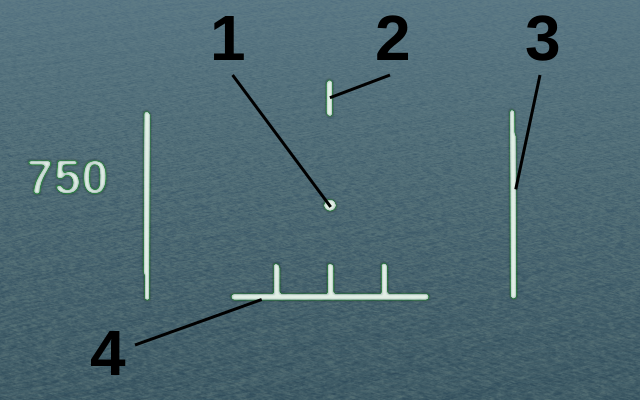
\includegraphics[width=0.45\textwidth]{images/displays/ajs-hud-aiming1.png}
  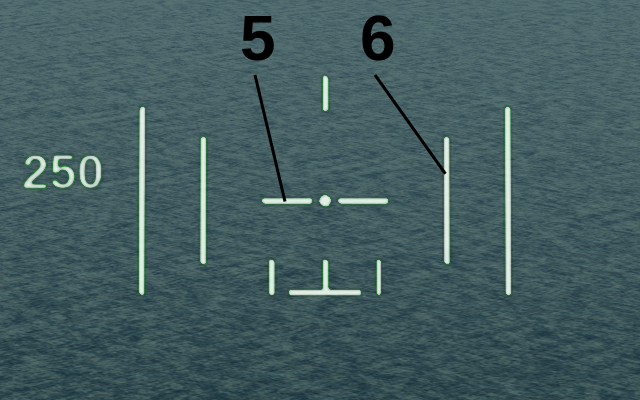
\includegraphics[width=0.45\textwidth]{images/displays/ajs-hud-aiming2.png}

  \begin{multicols}{2}
    \begin{enumerate}[nosep]
      \item \label{item:reticle} Aiming reticle
      \item \label{item:rdr-range} Radar ranging mark.
      \item Side bars, no functionality.
      \item \label{item:distline} Distance line.
      \item \label{item:fire-mark} Firing command lines.
      \item \label{item:pullup-bars} Evasion warning bars.
    \end{enumerate}
  \end{multicols}
  \caption{HUD aiming mode}
  \label{fig:hud-aiming}
\end{figure}

When AKAN or ARAK are selected, the HUD aiming mode (\cref{fig:hud-aiming})
is enabled by switching to mode ANF/CBT, or arming the weapon (trigger unsafe) in mode NAV.

It comports an aiming reticle (\figref{fig:hud-aiming}{item:reticle}),
the digital altitude indicator, and a number of indicators and cues for target range,
which appear in the following order:
\begin{enumerate}
  \item The distance line (\figref{fig:hud-aiming}{item:distline})
    indicates range to the target up to 8km when triangulation ranging is active.
    The side marks indicate the computed firing distance
    (minimum firing distance giving sufficient time for safe evasion).
  \item When radar ranging is active, a vertical bar is displayed above the reticle
    (\figref{fig:hud-aiming}{item:rdr-range}).
  \item 2 seconds before computed firing distance, the distance line blinks.
  \item 0.5 seconds before computed firing distance, the firing command lines appear
    (\figref{fig:hud-aiming}{item:fire-mark}).
  \item When the minimum distance for safe evasion is passed,
    the evasion warning bars start blinking (\figref{fig:hud-aiming}{item:pullup-bars}).
    This indicates that the attack run should be aborted immediately.
\end{enumerate}

Minimum distance for safe evasion is computed to keep the aircraft out of the
explosion debris zone, and assumes a 5g pull, with some margin.

The position of the aiming reticle is correct starting 3 seconds before computed firing distance.
The aiming reticle includes wind compensation.


\section{Rb 75}\label{sec:rb75}
The Rb 75 is a Swedish version of the AGM-65A television-guided missile.
It is designed for use against ground targets.
The pilot locks on the target by manually slewing the Rb 75 seeker head using the radar stick.

In the real Viggen, the EP-13 screen to the right of the HUD displayed the Rb
75 seeker image, and was used to lock on the target.

In FlightGear, the EP-13 screen is not functional.
Instead, the seeker position is displayed as a small circle on the HUD.
The seeker is controlled with the radar stick (see \cref{sec:cursor}):
\begin{itemize}[noitemsep]
  \item Initially, the seeker is locked straight ahead.
  \item Holding the radar stick trigger T1 (press \keys{\shift+O}) unlocks the seeker,
    which is then controlled with the radar stick.
  \item Releasing T1 (press \keys{\shift+O} again) re-centers the seeker.
  \item Pressing TV (\keys{L}) locks to a target. After lock, T1 can be released without losing lock.
  \item To unlock the seeker, release T1, then press it again.
\end{itemize}

\section{Rb 05A}
The Rb 05A is a remote-controlled missile.
It is primarily intended for use against ground and naval targets,
but can also be used against slow-manoeuvring air targets thanks to a proximity fuse.
The missile is guided visually by the pilot.
A flare at the back of the missile helps the pilot to keep sight of it (\cref{fig:rb05-flare}).

\begin{figure}
  \centering
  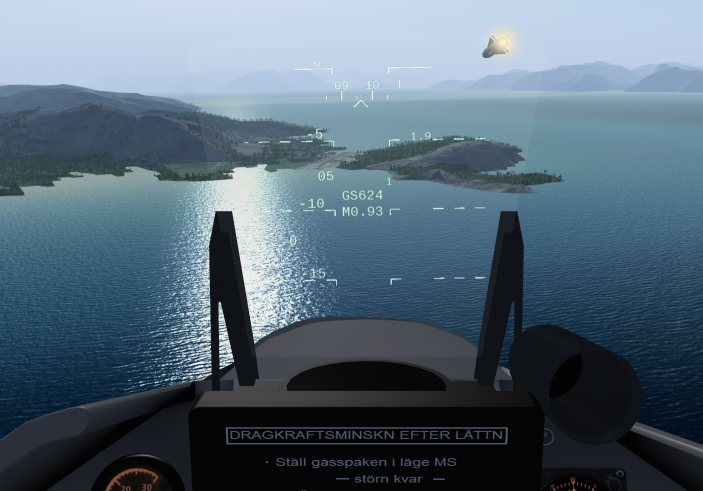
\includegraphics[height=0.3\textwidth]{images/weapons/rb_05a_start_popup.png}
  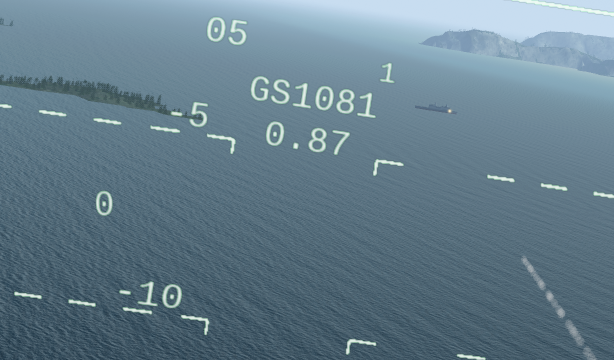
\includegraphics[height=0.3\textwidth]{images/weapons/rb_05a_before_impact_ship.png}
  \caption[Rb 05A flare for visual guidance]{Rb 05A flare for visual guidance.
    On the left, the missile is entering the pilot's field of view just after launch.
    On the right, the missile is about to hit the target ship,
    and the missile flare is visible over the ship
  }
  \label{fig:rb05-flare}
\end{figure}

In FlightGear, the Rb 05A uses the same controls as the radar stick, cf.\ \cref{sec:cursor}.\footnote{%
  In the real Viggen, a separate control stick on the right console was used.
}

\subsection{Procedure}
\begin{enumerate}
  \item Main mode selector to ANF/CBT.
    (\figref{fig:left-panel}{item:main-mode}, shortcuts \keys{M}/\keys{\shift+M}).
  \item Select the Rb 05A (cycle weapons with \keys{C}).
  \item Once in firing position, consider engaging autopilot in ATT or HÖJD/ALT mode to reduce pilot workload.
  \item Identify the target visually.
  \item Unsafe the trigger and fire within 9km of the target.
  \item After 1.7s, missile controls are enabled
    (cf.\ \cref{sec:cursor} for control methods).
    At this point, it should be well within the pilot field of view.
  \item When the missile hits, take evasive manoeuvres, secure the trigger, and switch to NAV mode.
\end{enumerate}

Remarks.
\begin{itemize}
  \item Recommended speed is 700--1150 km/h.
  \item Recommended attitude is a level flight or slight dive,
    so as to not loose sight of the target and the missile.
  \item Recommended altitude is 300--400 meters above ground.
  \item The target do not need to be directly in front of the aircraft
    as the missile can be guided considerably to the side.
    However, doing so makes it harder to aim the missile, and reduces effective range.
  \item The missile flies for ca.\ 24 seconds, giving it a maximum effective range of ca.\ 9 km.
  \item It is easiest to aim the missile using the collimation principle:
    try to keep the missile flare covering the target at all time.
\end{itemize}

\section{Rb-04E and Rb-15F}
These sea target missiles are fire and forget without locking on a target by the pilot.
The missiles will find their way to a target somewhat in the direction of the nose at release point.
The Rb-15F was also able to follow a preset route, this is not currently modelled.

The release range for the Rb-04E is between minimum 12km and maximum 24km;
for the Rb-15F it is up to 70km.
Sufficient release speed (around~M0.9) is important to reach maximum range.

To make sure that the missiles do not splash into the ocean after release:
\begin{itemize}
  \item The launch speed should be M0.7--M0.9.
  \item Drop altitude should be above 50 metres, i.e.\ you need to pop-up somewhat.
    According to the original manual for the Rb-04 you need to be between 50--425 metres (recommended 240).
    For the Rb-15 the aircraft needs to be between 50--2000 metres (recommended 600).
\end{itemize}

\section{m/90}
The Bombkapsel m/90 is gliding stand-off submunitions dispenser (cluster bomb) with 72 submunitions.
After release, it flies to and detonates over the current waypoint.
Thus,
\begin{itemize}
  \item Precise positioning of the waypoint is essential:
    consider doing a target fix (see \cref{sec:target-wpt}).
  \item The altimeter must be correctly set so that the m/90 aims for the correct altitude:
    set the altimeter to the target QFE, or switch the HUD to radar altimeter.
\end{itemize}

The m/90 can be released between 50 and 500 metres above terrain.
Its range depends on the speed and height of the launching aircraft and how much the m/90 needs to turn during gliding.
According to the original manual when releasing at 100 metres above terrain:
\begin{itemize}[nosep]
  \item At M0.7 the range is ca.\ 1.2--3km.
  \item At M0.9 the range is ca.\ 2--7km.
\end{itemize}
